\chapter{Discussion}\label{chap:DISCUSSION}
% ========================
We have considered two possibilities for this observable difference in the infrared colors of dwarf stars compared to giant stars. We have considered that the source of the color difference is due to (1) observational bias from reddening due to galactic extinction, or is (2) an astrophysical phenomenon that helps underline the intrinsic separation of dwarfs from giant stars. We stipulate that while there is a possibility both (1) and (2) could be contributing to the color difference we do see among different luminosity classes, it is more likely that (2) is the more dominant effect, which has interesting astrophysical implications in characterizing dwarfs from giants stars. We have examined the medians magnitudes of colors \jwone and \jwtwo across the galactic latitude coordinate $b$, and saw no strong dependence for $-15<b<15$ where extinction is greatest, and may have contributed more reddened colors that could have explained this difference (Figure \ref{fig:color-vs-b}).

\begin{figure}
    \centering
    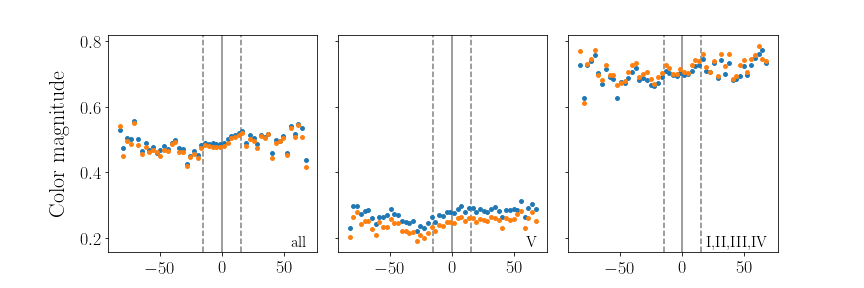
\includegraphics[width=1.0\textwidth,clip=true]{Figures/populations/plot-b-vs-color.png}
    \caption{This figure displays the median values of color magnitude \jwone and \jwtwo across galactic latitude for different luminosity classes. Colors magnitude and luminosity class information originate from a cross-matched table of WISE/2MASS with the Michigan Spectral Atlas, and no extinction correction has been applied. When calculating median value from the observed color magnitude, we created two different groups according to luminosity class: $V$ as dwarfs, and all other luminosity classes ($I$, $II$, $III$, $IV$) as giants. As expected, giants are redder than dwarfs on average for all galactic latitudes. We estimate that any reddening effect due to extinction should be strongest at the sky area that covers the galactic plane where gas clouds are concentrated, at approximately $-15<b<15$. Median color does not typically spike in the galactic plane for both \jwone and \jwtwo while in the same group, which suggests that the color separation between dwarfs and giants is not due to extinction, but from astrophysical phenomenon, such as gravity-sensitive lines in J-band.}
    \label{fig:color-vs-b}
\end{figure}

Therefore J is just damn special, and it would be a subject of future work as to why J band spectral features are gravity sensitive for GKM dwarfs (J-K for M dwarfs) and J-W1/2 for GK dwarfs.

We also note the importance the J-band is in differentiating between dwarfs from giants given its previously proved sensitivity for differentiating M dwarfs from GK dwarfs for J-K (REF). The combination of this study with J-W1/2 in being sensitive for GK dwarfs, and J-K being sensitive for GKM stars suggests the presence of surface gravity sensitive lines in the J-band. Thus, there we suggest it is viable to search for gravity sensitive lines along these the J-band wavelength range.